\section{Ziel}
\label{sec:Ziel}
Bei diesem Versuch werden die Eigenschaften von Operationsverstärkern untersucht. 
Dafür werden Operationsverstärker in verschiedene Schaltungen eingebaut und ihre Funktionsweise getestet.

\section{Theorie}
\label{sec:Theorie}
Operationsverstärker sind Differenzverstärker, d.h. die Ausgangsspannung $U_A$ ist proportional zu der Differenz der beiden Eingangsspannungen $U_P$, $U_N$

\begin{equation*}
    U_A = V \cdot (U_P - U_N).
\end{equation*}
Somit ist die Ausgangsspannung in der Phase der am nicht-invertierenden Eingang (+) anliegenden Spannung $U_P$ und gegenphasig zur am invertierenden Eingang (-) anliegenden Spanung $U_N$.
Das proportionale Verhalten der Ausgangsspannung gegenüber der Differenz der beiden Eingangsspannungen, besteht nur im Bereich 

\begin{equation*}
    -U_S < U_A < U_S,
\end{equation*}
wobei $U_S$ die angelegte Betriebsspannung ist.
Außerhalb dieses Bereiches entspricht die Ausgangsspannung $\pm U_S$.
%Ein solcher Operationsverstärker ist in Abbildung \ref{fig:1} gezeigt.

%\begin{figure}
%    \centering
%        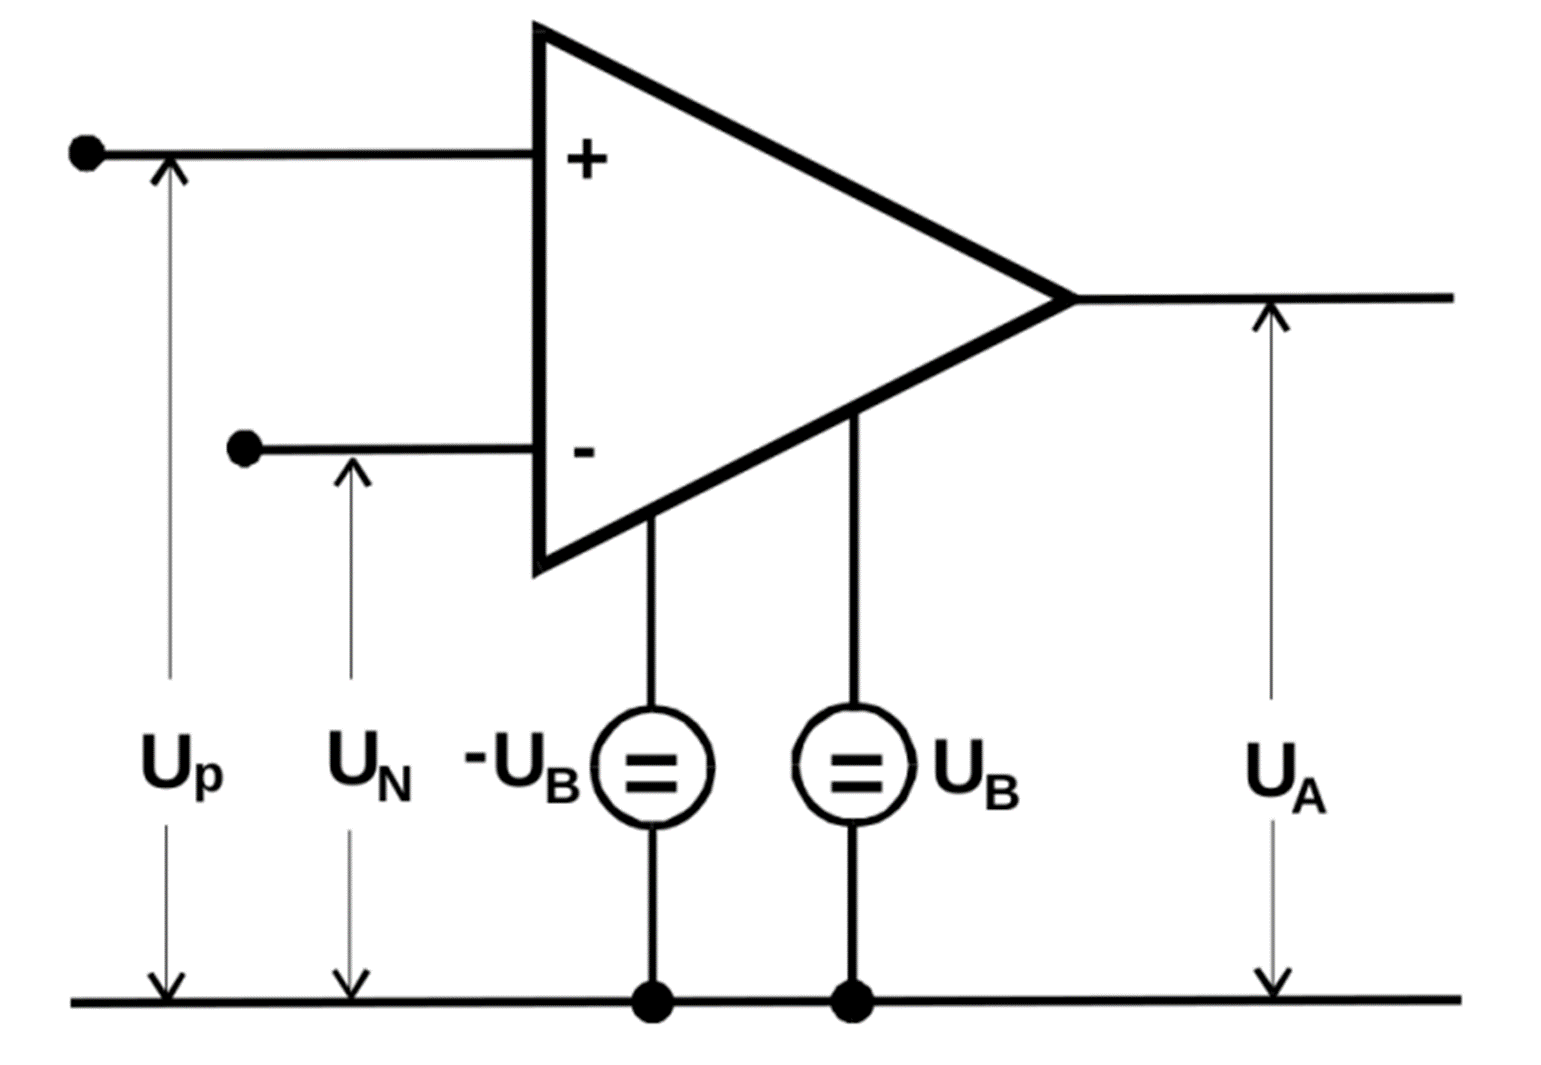
\includegraphics[width= \textwidth]{plots/OP.png}
%    \caption{Schematische Darstellung eines Operationsverstärkers \cite{Anleitung}.}
%    \label{fig:1}
%\end{figure}


Der ideale Operationsverstärker hat eine Leerlaufverstärkung von $V \rightarrow \infty$.
Zudem sind die Eingangswiderstände $r_p$ und $r_n$ ebenfalls unendlich groß und der Ausgangswiderstand $r_a = 0 \Omega$.
Es werden Signale jeglicher Frequenz übertragen.

Diese Bedingungen lassen sich bei einem realen Operationsverstärker nicht umsetzen.
Dies führt zu einer Leerlaufverstärkung von $V \propto 10^4 - 10^6$ und einer Übertragingsbandreite von $\SI{10}{\hertz}$ bis $\SI{10}{\kilo\hertz}$.
Zusätzlich entsteht eine geringe Gleichtaktverstärkung, so wie eine Offsetspannung, wenn beide Eingangsspannungen 0 $V$ betragen.
Diese Offsetspannung ist als

\begin{equation*}
    U_0 = U_P - U_N
\end{equation*}
definiert, wobei die Eingangsspannungen so gewählt sind, dass $U_A = 0$.



\subsection{Schaltungen mit Operationsverstärkern}
\label{sec:Schaltungen}

\subsubsection{Invertierender Linearverstärker}
\label{sec:Invertierter_Linearverstärker}

In Abbildung \ref{fig:2} ist ein invertierter Linearverstärker gezeigt. 
Bei diesem wird die Ausgangsspannung über den Widerstand $R_2$ in den invertierenden Eingang des Operationsverstärkers gegeben. 
Dadurch kommt es bei einer Zunahme der Ausgangsspannung zu einer Abnahme der Eingangsspannung.
Diese Gegenkopplung wirkt einer Ausgangsspannung im gesättigten Bereich entgegen.

\begin{figure}
    \centering
        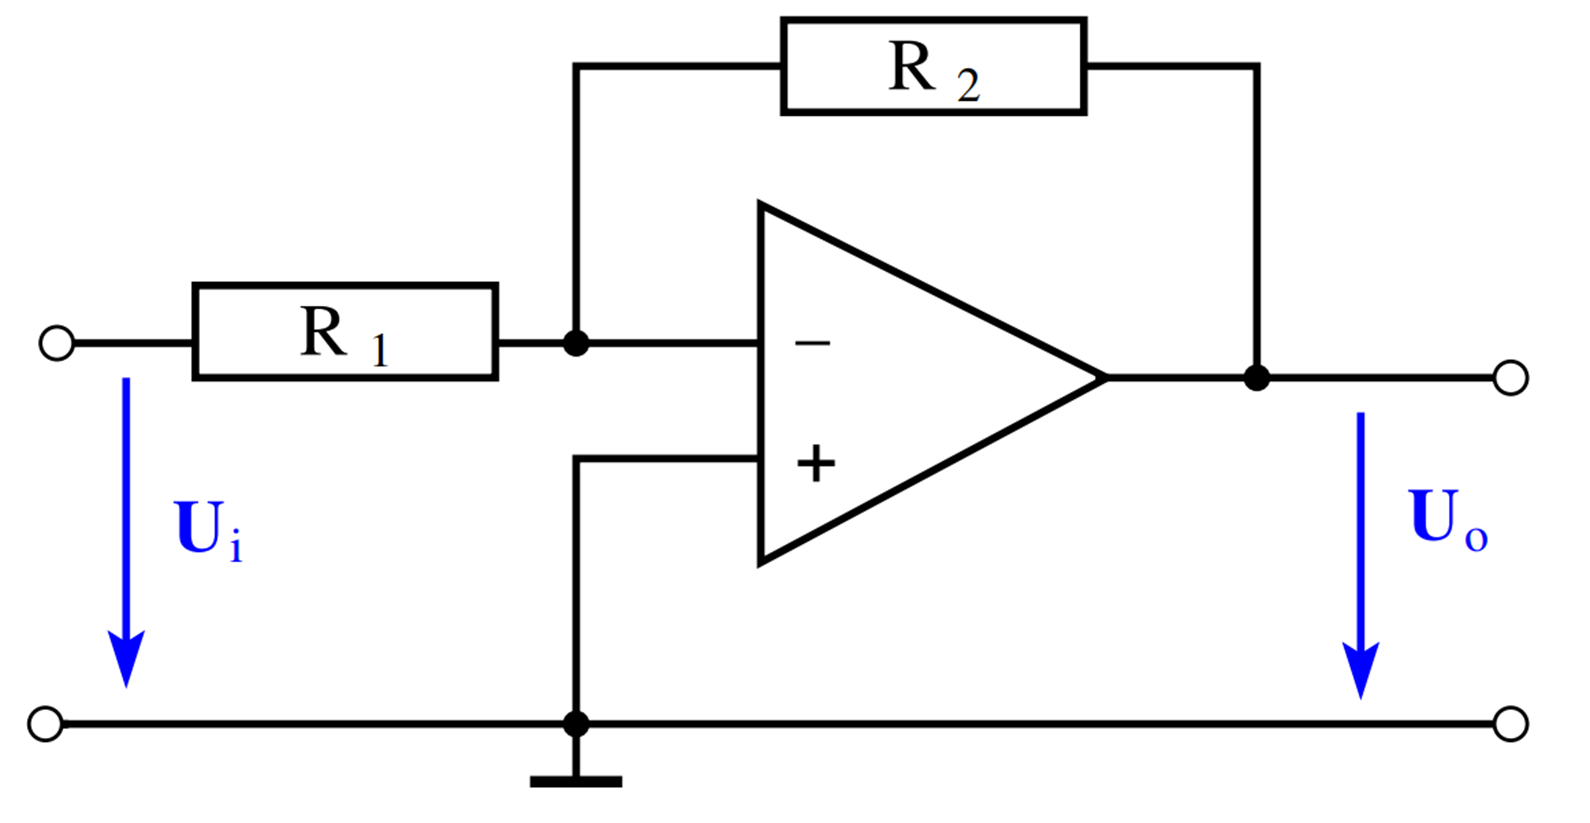
\includegraphics[width= 0.6\textwidth]{plots/Verstärker.png}
    \caption{Schematische Darstellung eines invertierenden Verstärkers \cite{Anleitung}.}
    \label{fig:2}
\end{figure}

Aus der Proportionalität der Ausgangsspannung zur Eingangsspannung ergibt sich 

\begin{equation}
    \label{equ:1}
    U_N = - \frac{U_A}{V}.
\end{equation}
Mit der Annahme $I_N = 0$, folgt aus der Knotenregel für den Knoten vor dem invertierenden Eingang

\begin{equation}
    \label{equ:2}
    \frac{U_N - U_1}{U_A - U_1} = \frac{R_1}{R_1 + R_N}.
\end{equation}
Unter Berücksichtigung von Formel \eqref{equ:1} und \eqref{equ:2}, so wie der Näherung $V >> 1$ ergibt sich

\begin{equation}
    \frac{1}{V^{'}} = \frac{1}{V} + \frac{R_1}{R_N}.
\end{equation}
Gut zu sehen ist, dass die Verstärkung bei $\frac{R_N}{R_1} << V$ nahezu nur noch von dem Verhältnis der Widerstände abhängt.
Diese Gegenkopplung verringert damit die starken schwankungen von $V$ und erhöht so die Stabilität des Verstärkers.



\subsubsection{Umkehrintegrator}
\label{sec:Umkehrintegrator}

Tauscht man den Widerstand in der Rückkopplung des invertierenden Linearverstärker durch einen Kondensator, so erhält man einen Umkehrintegrator.
Dieser ist in Abbildung \ref{fig:3} dargestellt.

\begin{figure}
    \centering
        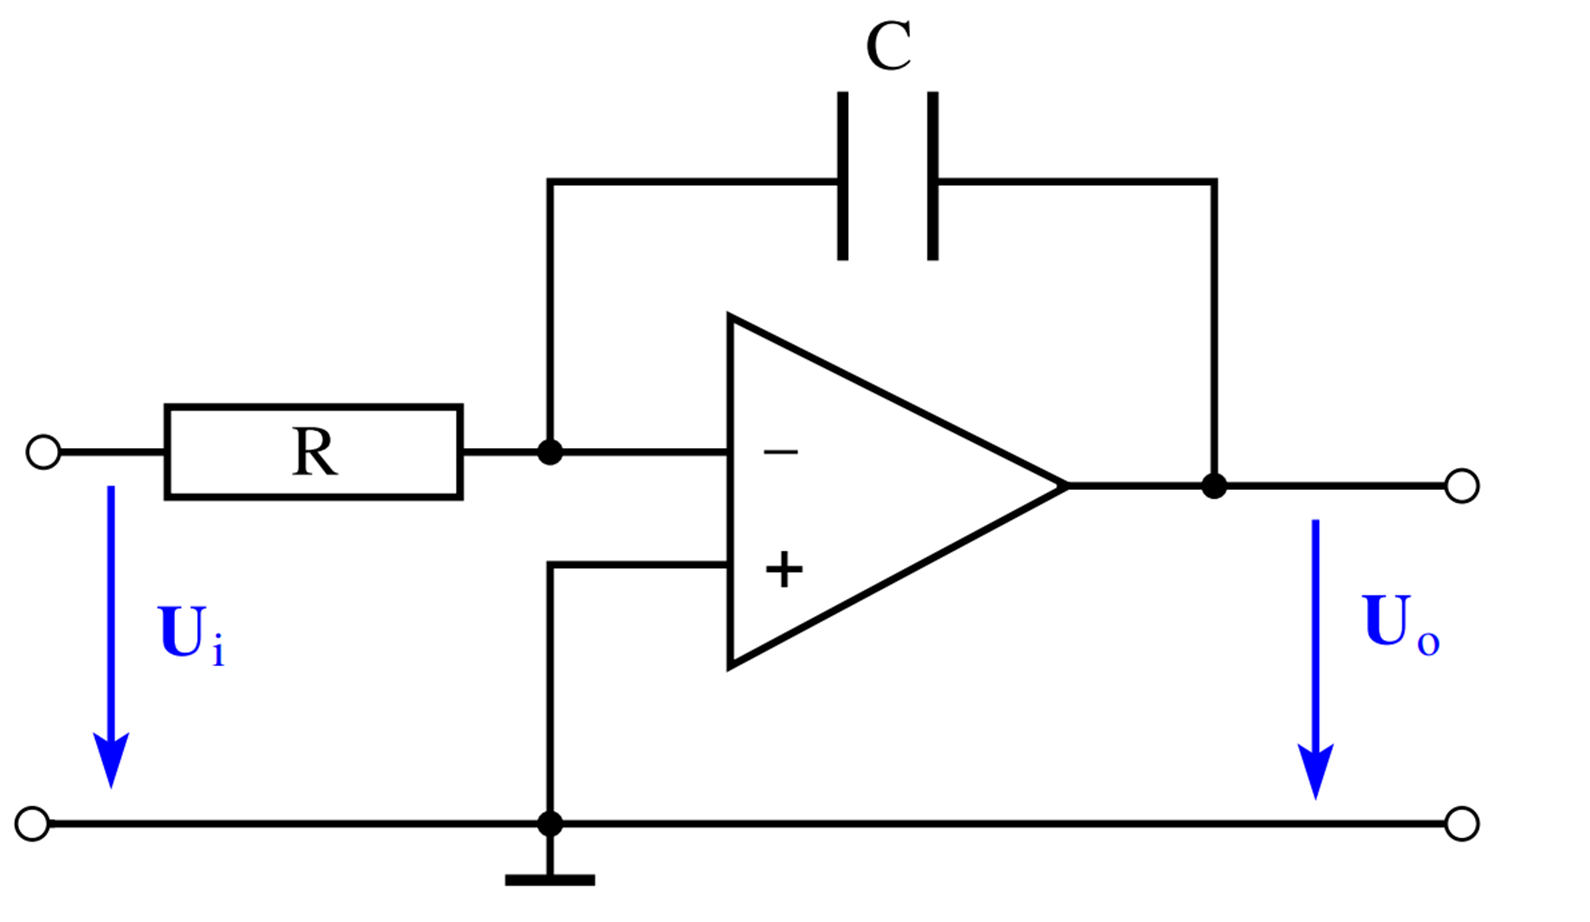
\includegraphics[width= 0.6\textwidth]{plots/Integrator.png}
    \caption{Schematische Darstellung eines Umkehrintegrators \cite{Anleitung}.}
    \label{fig:3}
\end{figure}

Durch die Knotenregel und der Näherung $I_N = 0$, ergibt sich für den Knoten vor dem invertierenden Eingang

\begin{equation}
    I_1 + I_C = 0.
\end{equation}
Weiterhin gilt

\begin{equation}
    I_1 = \frac{U_1}{R_1},
\end{equation}
so wie

\begin{equation}
    \int I_C \text{d}t = C U_A.
\end{equation}
Daraus berechnet sich die Ausgangsspannung zu 

\begin{equation}
    U_A = -\frac{1}{R C} \int U_1 \text{d}t.
\end{equation}
Für eine sinusförmige Eingangsspannung $U_! = U_0 \text{sin}(\omega t)$ folgt nun

\begin{equation}
    U_A = - \frac{U_0}{R C \omega} \text{cos}(\omega t).
\end{equation}



\subsubsection{Invertierender Differentiator}
\label{sec:Invertierter_Differentiator}

Werden nun der Widerstand und der Kondensator des Umkehrintegrators vertauscht, so eintsteht der invertierende Differentiator, abgebildet in Abbildung \ref{fig:4}.

\begin{figure}
    \centering
        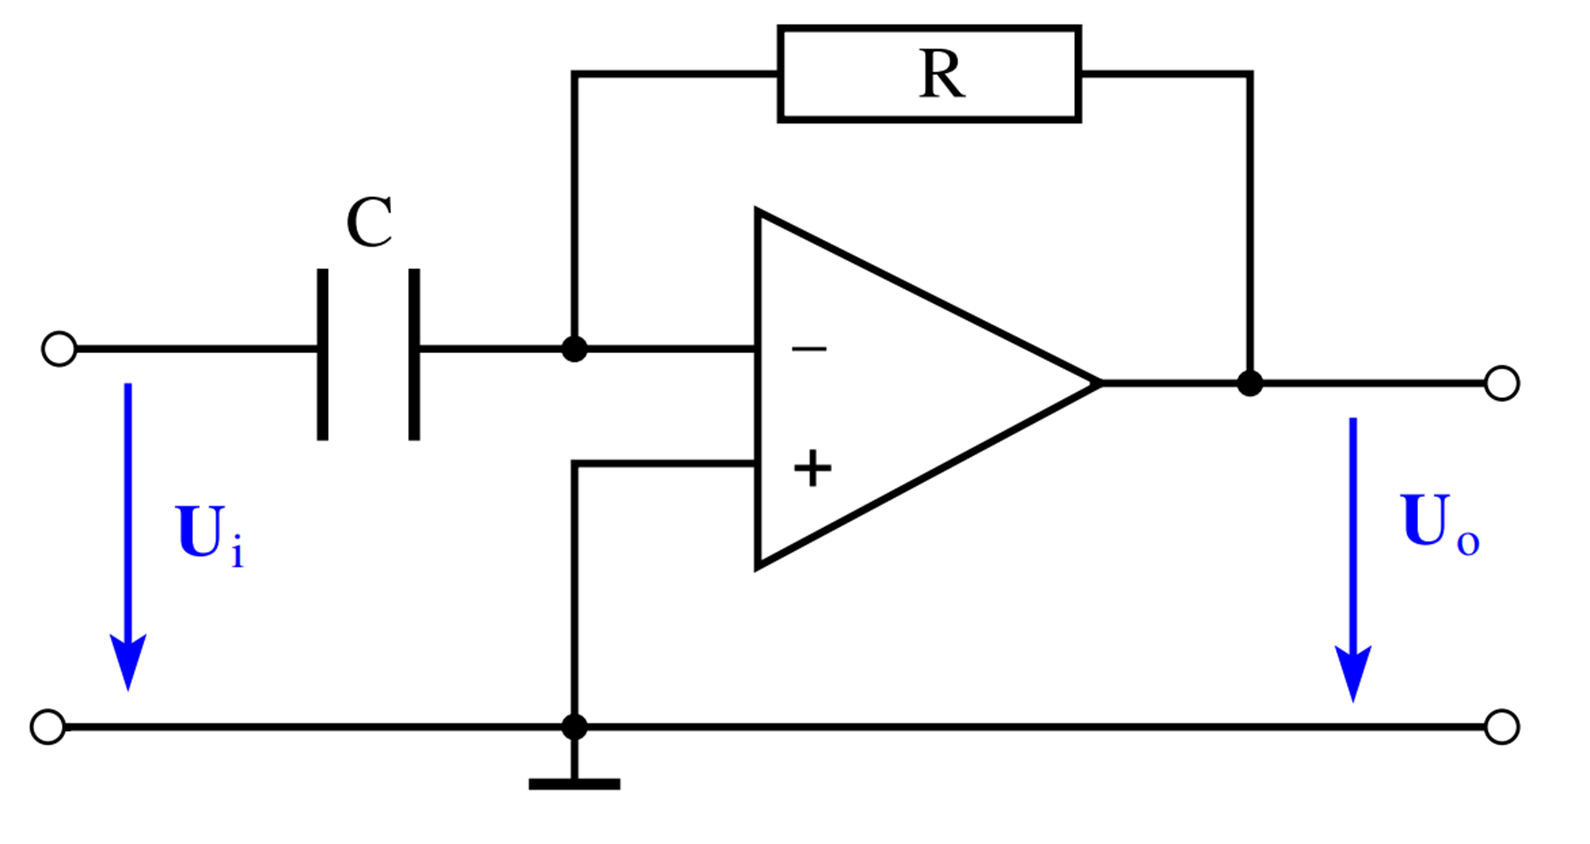
\includegraphics[width= 0.6\textwidth]{plots/Differentiator.png}
    \caption{Schematische Darstellung eines invertierten Differentiators \cite{Anleitung}.}
    \label{fig:4}
\end{figure}

Für den Knoten vor dem invertierenden Eingang ergibt sich dann

\begin{equation*}
    I_1 + I_A = 0,
\end{equation*}
mit den Strömen

\begin{align*}
    I_1 = \dot Q = C \cdot \dot U_1 \\
    I_A = \frac{U_A}{I_A}.
\end{align*}
Damit hängt die Ausgangsspannung von der zeitlichen Ableitung der Eingangsspannung ab

\begin{equation*}
    U_A = -R C \cdot \dot U_1.
\end{equation*}
Für eine Eingangsspannung $U_1 = U_0 \text{sin} (\omega t)$ ergibt sich dann die Ausgangsspannung 

\begin{equation}
    U_A = -RC U_0 \omega \cdot \text{cos} (\omega t),
\end{equation}
welche proportional zur Frequenz ist.



\subsubsection{Schmitt-Trigger}
\label{sec:Schmitt-Trigger}


Bei dem Schmitt-Trigger, gezeigt in Abbildung \ref{fig:5}, wird das Ausgangssignal über einen Widerstand in den nicht invertierenden Eingang des Operationsverstärkers gegeben.
Dadurch wird das Eingangssignal verstärkt, wodurch der Schmitt-Trigger einem Schalter ähnelt.
Übersteigt die Spannungsdifferenz an den Eingängen einen bestimmten Schwellenwert, so springt die Ausgangsspannung schlagartig auf $\pm U_S$.
Daraus ergibt sich die rechteckige Ausgangsspannung.
Die Schwellenwerte sind gegeben durch $- \frac{R_1}{R_P} U_S$ und $\frac{R_1}{R_P} U_S$.

\begin{figure}
    \centering
        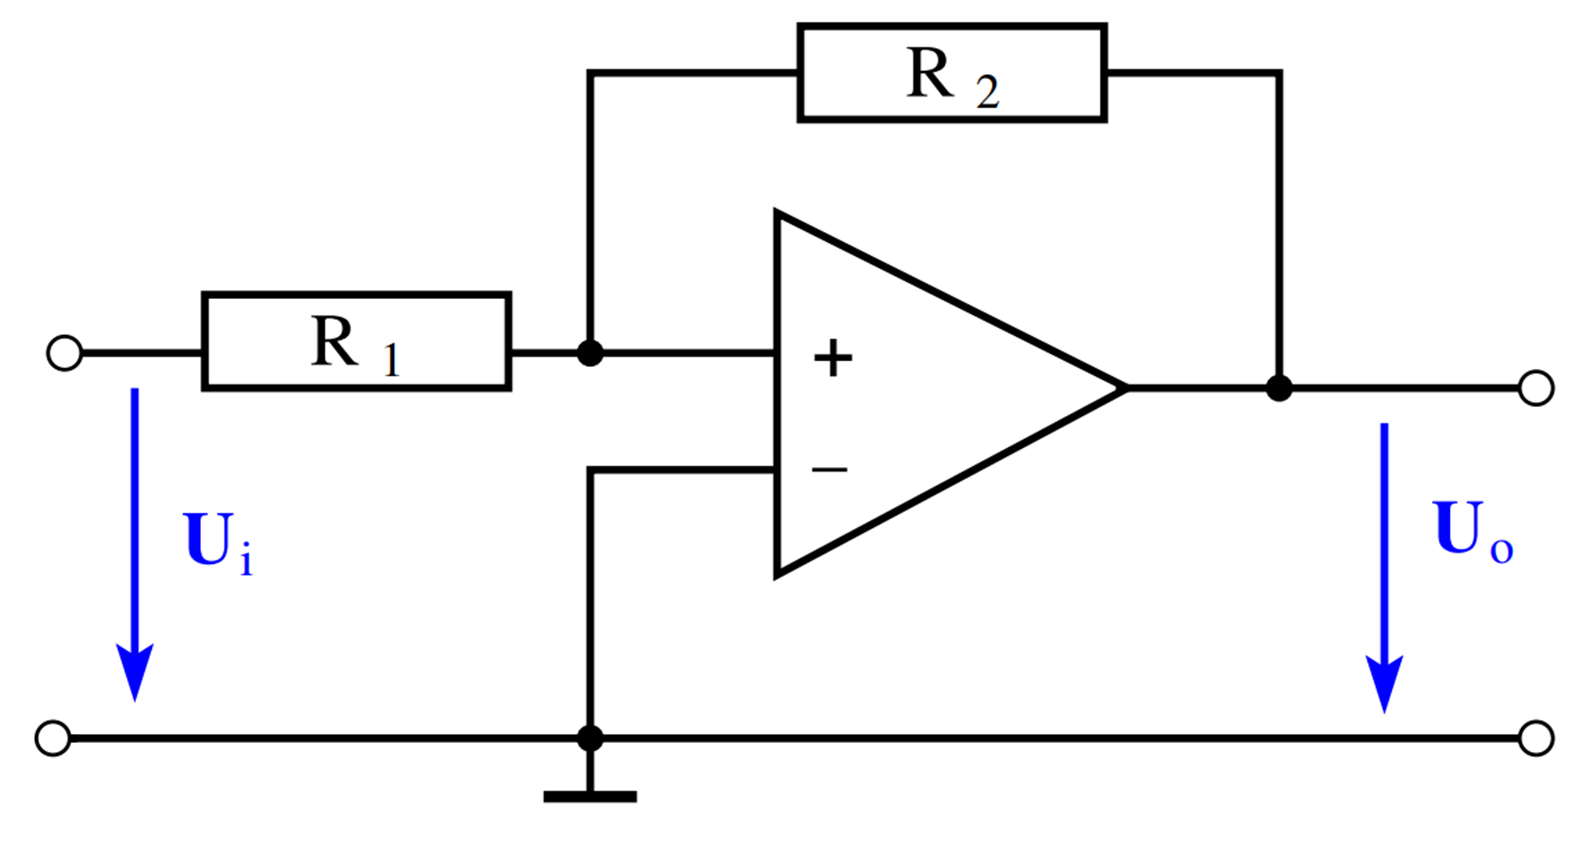
\includegraphics[width= 0.6\textwidth]{plots/Schmitt.png}
    \caption{Schematische Darstellung eines Schmitt-Triggers \cite{Anleitung}.}
    \label{fig:5}
\end{figure}

\subsubsection{Signalgenerator}
\label{sec:Signalgenerator}

Die Kombination aus Schmitt-Trigger und Integrator ist in Abbildung \ref{fig:6} dargestellt und entspricht einem Signalgenerator, welcher spontan anfängt zu schwingen.
Die Rechtecksspannung am Ausgang des Schmitt-Triggers wird durch den Integrator integriert, was zu einer Dreiecksspannung am Ausgang des Integrators führt.
Diese Dreiecksspannung wird wiederum als Eingangsspannung für den Schmitt-Trigger genutzt.
Die Frequenz des schwingenden Systems ergibt sich zu $\nu_{\text{Dreieck}} = \frac{R_2}{4 C R_1 R_3}$ und die Amplitude entspricht $A = U_{\text{max}} \frac{R_q}{R_2}$.

\begin{figure}
    \centering
        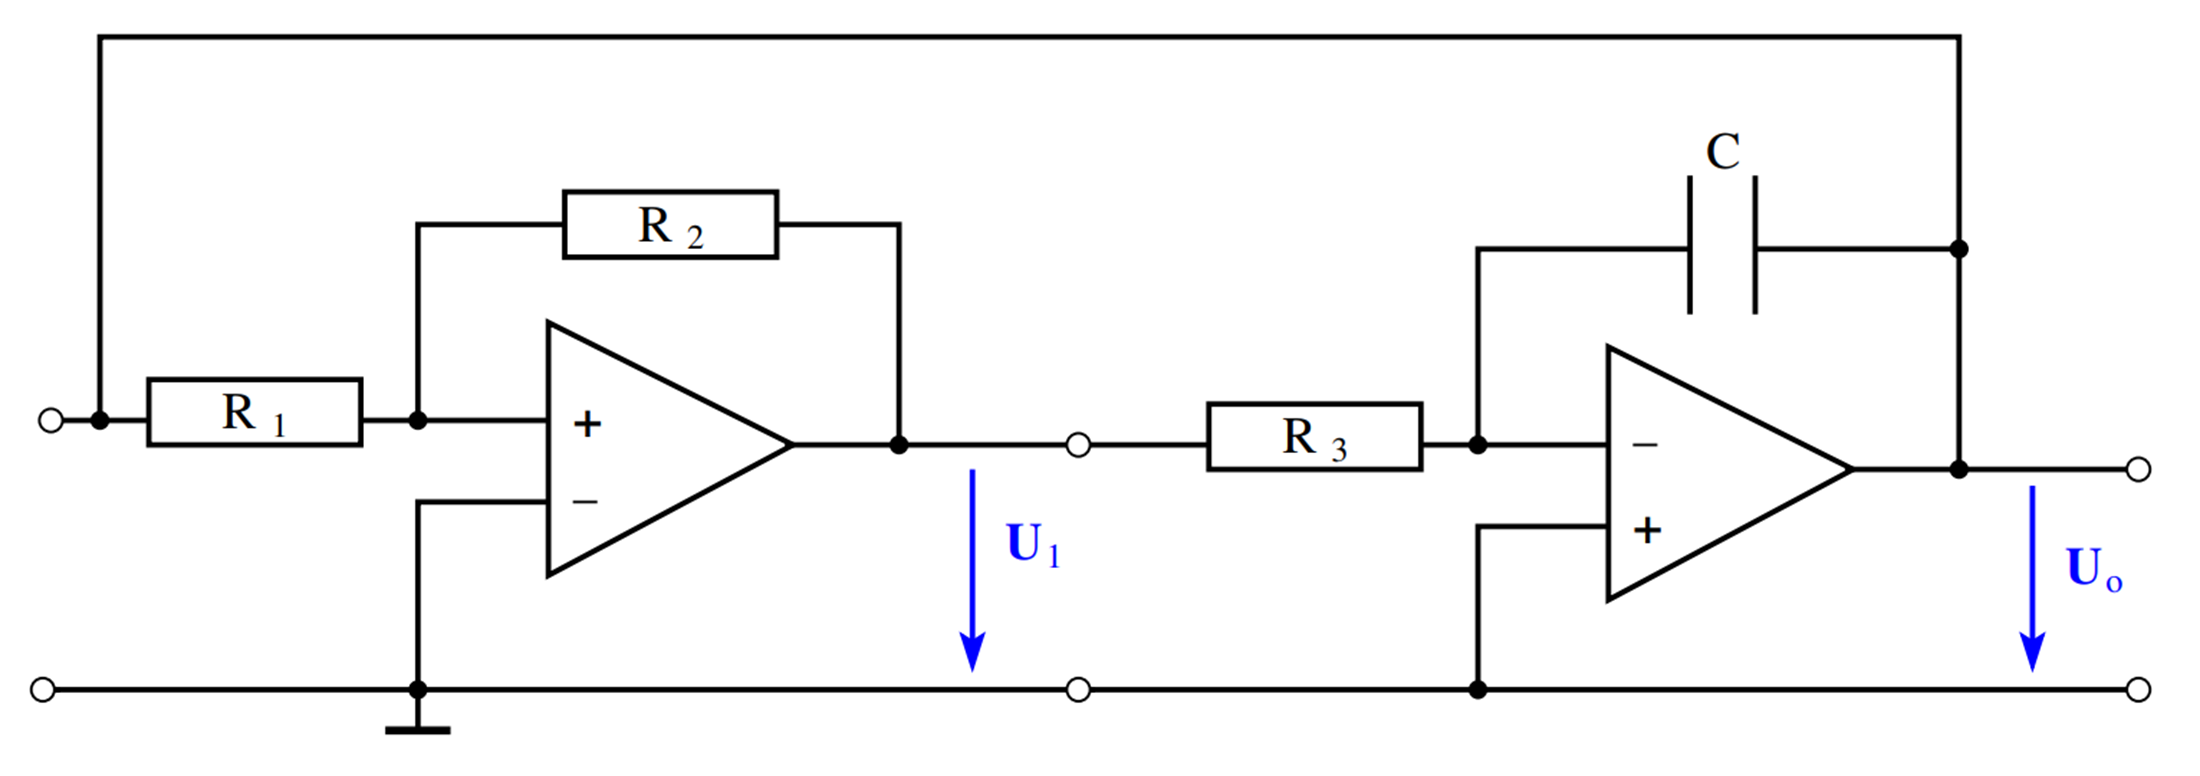
\includegraphics[width= 0.7\textwidth]{plots/Generator.png}
    \caption{Schematische Darstellung eines Signalgenerators \cite{Anleitung}.}
    \label{fig:6}
\end{figure}


\subsubsection{Signalgenerator mit variierenden Amplituden}
\label{sec:Signalgenerator_2}

Durch den in Abbildung \ref{fig:7} gezeigten Aufbau kann durch eine am Eingang anliegende Rechtecksspannung, eine gedämpfte Schwingung erzeugt werden.
Diese gedämpfte Schwingung hat die Periodendauer 

\begin{equation}
    T = 2 \pi R C
\end{equation}
und eine Zerfallszeit von

\begin{equation}
    \tau = \frac{20 R C}{|\rho|}.
\end{equation}
Dabei gilt für die Konstante $\rho$ doe Bedingung $-1 \leq \rho \leq 1$.
\begin{figure}
    \centering
        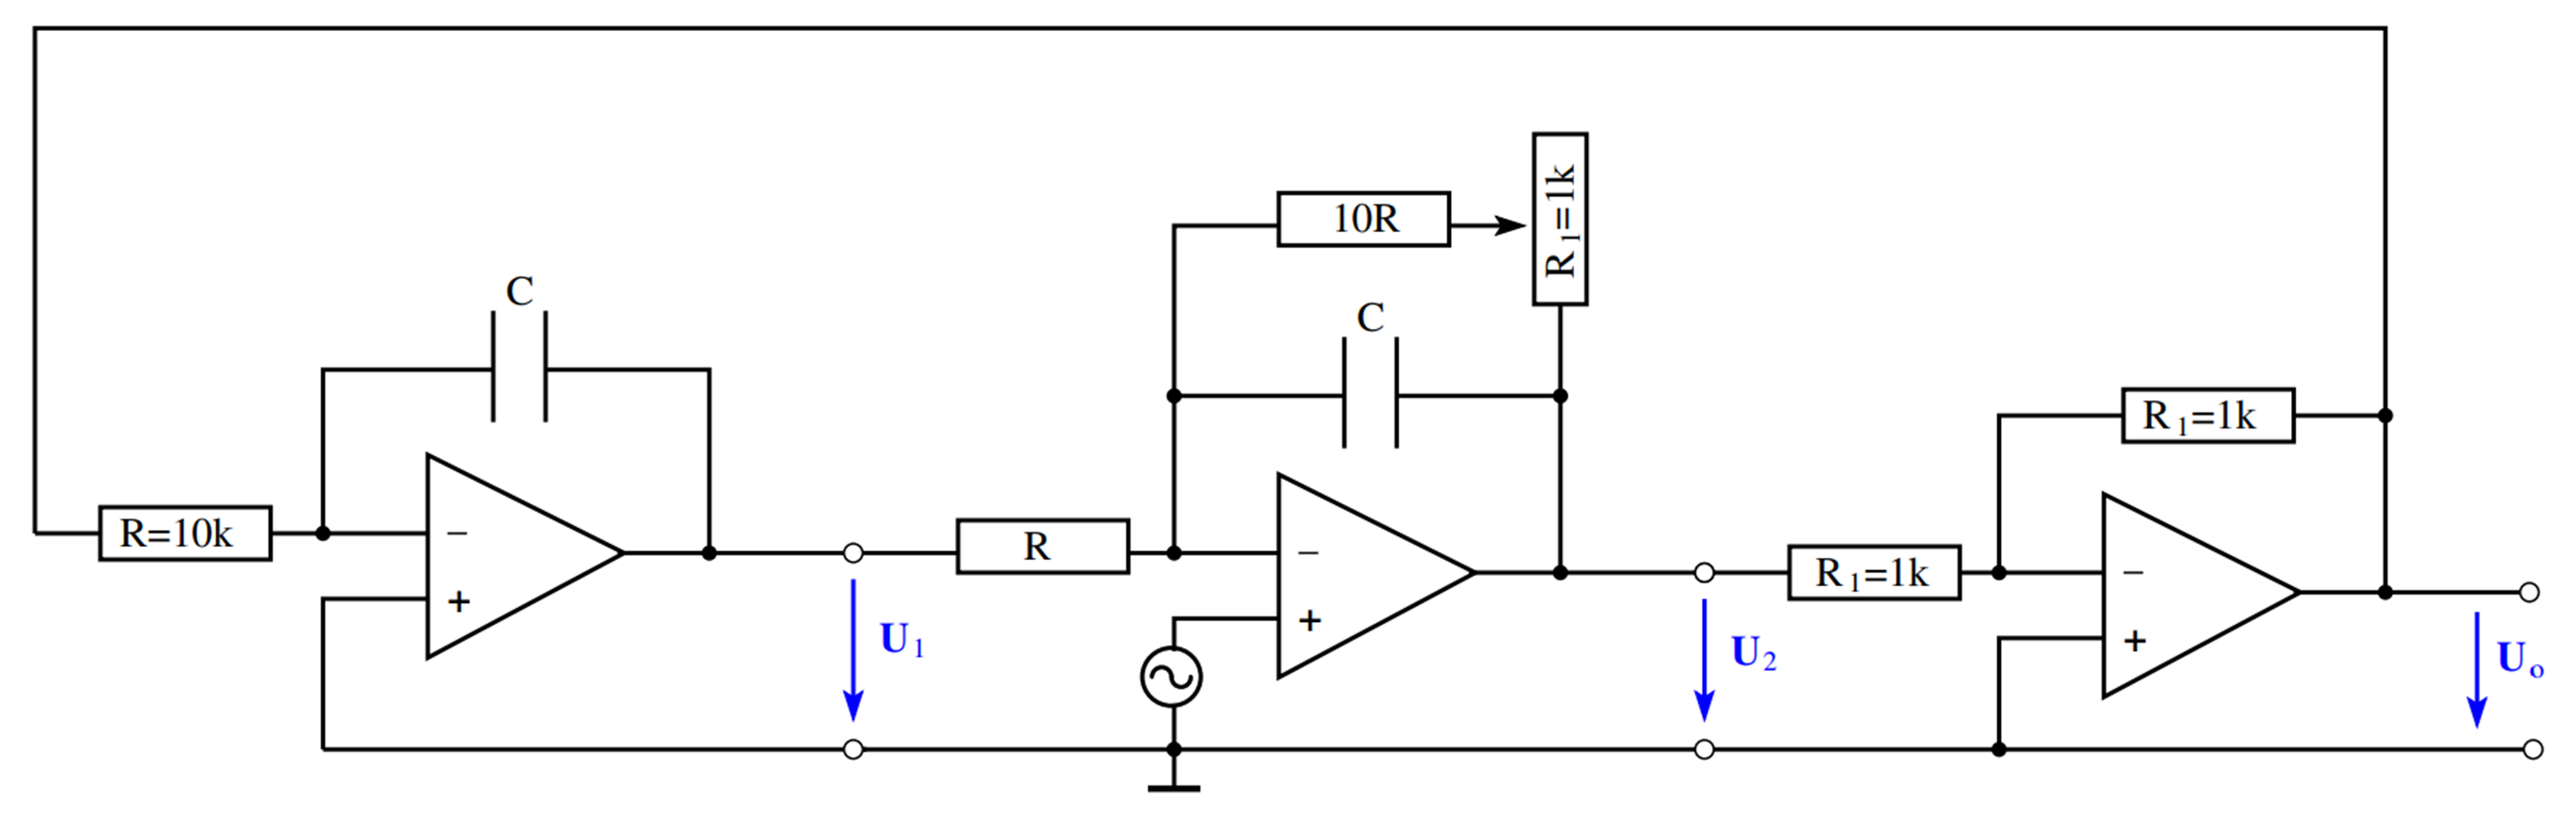
\includegraphics[width= 0.8\textwidth]{plots/Schwingung.png}
    \caption{Schematische Darstellung eines Signalgenerators mit variierender Amplitude \cite{Anleitung}.}
    \label{fig:7}
\end{figure}